\documentclass{article}

\usepackage[letterpaper, margin=1in]{geometry}

\usepackage{lineno}
\linenumbers
\usepackage{titlesec}
%\usepackage[none]{hyphenat} % use only if there is a problem
% Use Unicode characters
\usepackage[utf8]{inputenc}

\usepackage{scicite}
% Clean citations with biblatex
\usepackage[
backend=biber,
style=science
]{biblatex}

\addbibresource{zotero.bib}

% Highlighting
\usepackage{color}
\usepackage{soul}
\usepackage{xurl}

% tables
\usepackage{longtable,booktabs,array}
\usepackage{multirow}
\usepackage{afterpage}

% figures
\usepackage{wrapfig}
\usepackage{lscape}
\usepackage{rotating}
\usepackage{graphicx}
\graphicspath{assets}
\usepackage{times}
\usepackage{caption}


\topmargin 0.0cm
\oddsidemargin 0.2cm
\textwidth 16cm 
\textheight 21cm
\footskip 1.0cm

\title{Supplementary material for "Gut microbes and their genes are associated with cognition and neuroanatomy in children"}

\begin{document}

\baselineskip24pt

\maketitle

\begin{figure}[!htb]
    \centering
    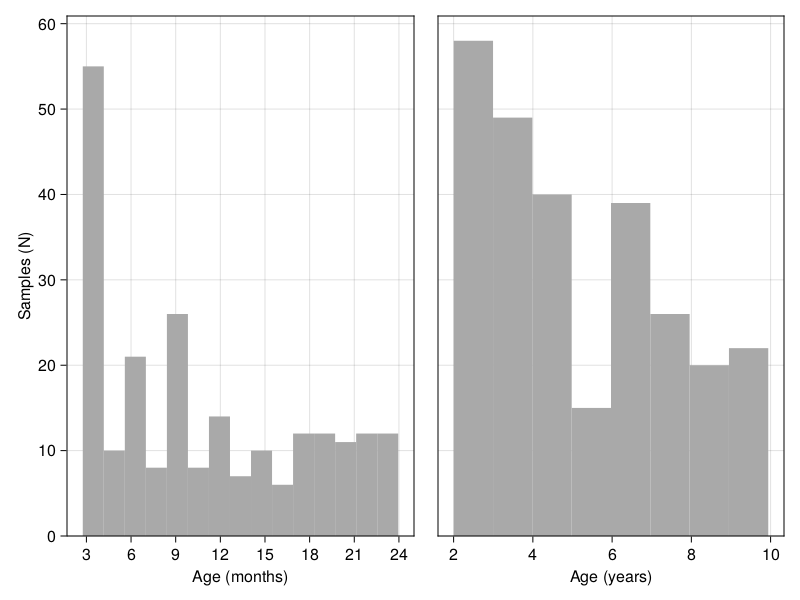
\includegraphics[width=0.9\textwidth]{assets/Supp_Figure1.png}
    \captionsetup{labelformat=empty}
    \caption{
        \textbf{Figure S1}: Sample collection by age - related to Figure 1A. A histogram showing the number of samples
        included in this study by the age of the child when the sample was collected.
    }
\end{figure}

\begin{figure}[!htb]
    \centering
    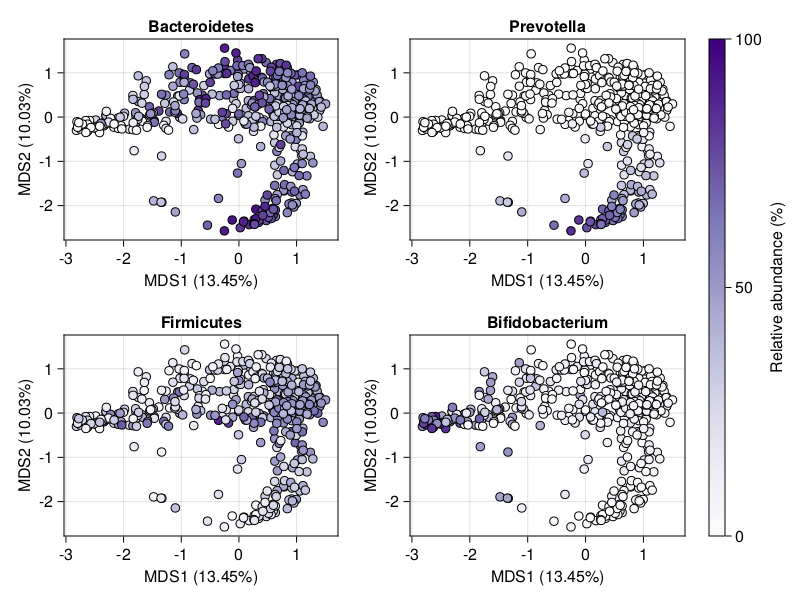
\includegraphics[width=0.9\textwidth]{assets/Supp_Figure2.png}
    \captionsetup{labelformat=empty}
    \caption{
        \textbf{Figure S2}: Principal coordinates analysis of taxonomic profiles - 
        related to Figure 1C. PCoAs are colored by the relative abundance per-sample
        of major phyla (Bacteroidetes, top left; Firmicutes, bottom left)
        and genera (\textit{Prevotella}, top right; \textit{Bifidobacterium}, bottom right).
    }
\end{figure}


\begin{figure}[!htb]
    \centering
    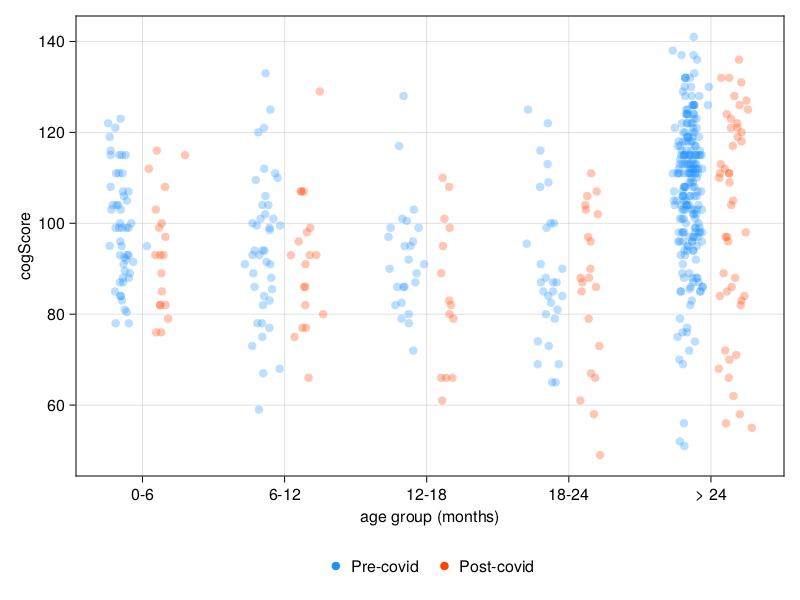
\includegraphics[width=0.9\textwidth]{assets/Supp_Figure3.png}
    \captionsetup{labelformat=empty}
    \caption{
        \textbf{Figure S3}: Cognitive assessment scores based on age
        and COVID-19. Scores in red were collected after March of 2020.
    }
\end{figure}


\end{document}